\documentclass[a4paper,10.5pt]{ltjsarticle}
\usepackage{graphicx}
\usepackage{caption}
\usepackage{luatexja-fontspec}
\usepackage[top=10truemm,bottom=15truemm,left=10truemm,right=10truemm]{geometry}
\usepackage{array}
\usepackage{upgreek}
\usepackage{braket}
\usepackage{fancyhdr}
\renewcommand{\refname}{}
\captionsetup[figure]{format=plain, labelformat=simple, labelsep=quad, font=bf}
\captionsetup[table]{format=plain, labelformat=simple, labelsep=quad, font=bf}
\parindent = 0pt
\setmainjfont[BoldFont=HiraMinProN-W6]{HiraMinPro-W3}
%[BoldFont=HGSMinchoE]{MSMincho}[BoldFont=HiraMinProN-W6]{HiraMinPro-W3}
\begin{document}

\centerline
{\huge \bfseries 調査}
\rightline
{May/09/2024}
\leftline
{}
\leftline{\large \bfseries 動向}\\
・Most commonly, atoms from the first two groups of the periodic table are used, since these are well- suited for cooling and trapping due to their electronic structure Ref\cite{1}.\\
・中性原子の計算速度を早くするために、gateを並列して作用させる動きが強まっているRef\cite{1}。\\
・quantum memoryというcontextで、malti-level qubitが研究されているRef\cite{2}。\\
\\
\leftline{\large \bfseries わかっていること}\\
・Superconductors: This approach uses superconducting resonant circuits to build qubits. The circuits operate at very low temperatures, allow for fast gate operations, but currently still suffer from low coherence times and limited connectivity.\\
・Ion traps: These use trapping techniques to trap ions in a vacuum chamber, laser cooling techniques to cool the ions, and electromagnetic pulses in the optical, microwave, or radio frequency range to manipulate their quantum states. This approach has been successfully used to manufacture quantum computers with high levels of coherence and very high connectivity. However, calculation speed and scaling to large numbers of qubits remain a challenge.\\
・Neutral atoms: This approach uses laser cooling and trapping techniques for neutral atoms and manipulates their quantum states using optical or microwave pulses. It offers long coherence times, scaling in 2D or even 3D, and fair connectivities by long-range interactions (Rydberg states). The main challenges include further improvement of the two-qubit gate fidelities and gate operation speeds.\\
・Photons: Photonic quantum computers use light to carry quantum information, which promises very good scalability. The virtually non-existent interaction between photons imposes a challenge to implementing gate operations. Thus, most often, so-called measurement-based quantum computing is being used.\\
・Spins in semiconductors: In this approach, the spin of electrons or nuclei, typically in silicon, is used as the basis for qubits. It is compatible with existing semiconductor fabrication techniques, making it a promising option for scaling. However, the feasibility of such scaling concepts still has to be shown.\\
・NV centers in diamond: This approach uses nitrogen-vacancy (NV) centers in diamond to create qubits. The NV center is a defect that is usually manipulated using laser techniques and—at least theoretically—offers room-temperature operation.\\
・Cold atom-based systems typically work at room temperature, but the atoms themselves are cooled to below 1 mK using laser light Ref\cite{1}.\\
・中性原子の測定は、$\ket{1}$のみを光によってぶっ飛ばし、黒い点(何もない)になったところが$\ket{1}$、光続けているところを$\ket{0}$とするRef\cite{1}。\\
・中性原子ではsingle gateを複数のqubitに対して同時に作用させることができるRef\cite{1}。\\
・Rydberg stateを用いると、connectivityを最大で1:50にすることができるRef\cite{1}←!?\\
・Rydberg stateはstrong dipole momentを使うためノイズに弱い。\\
・The depth of the traps can be increased by changing the frequency detuning of the laser light to be closer to the atomic transition. As this in turn leads to shorter T1 decoherence times, a trade-off between these effects has to be found.\\
・cryostats might be used in the future to increase the qubit lifetimes, providing on-premise access to neutral atom quantum computers or integrating them into classical supercomputing centres seems to be well possible in the near future.\\
\clearpage
・現時点(in 2023)での中性原子の性能Ref\cite{1}
\begin{figure}[h]
  \centering
  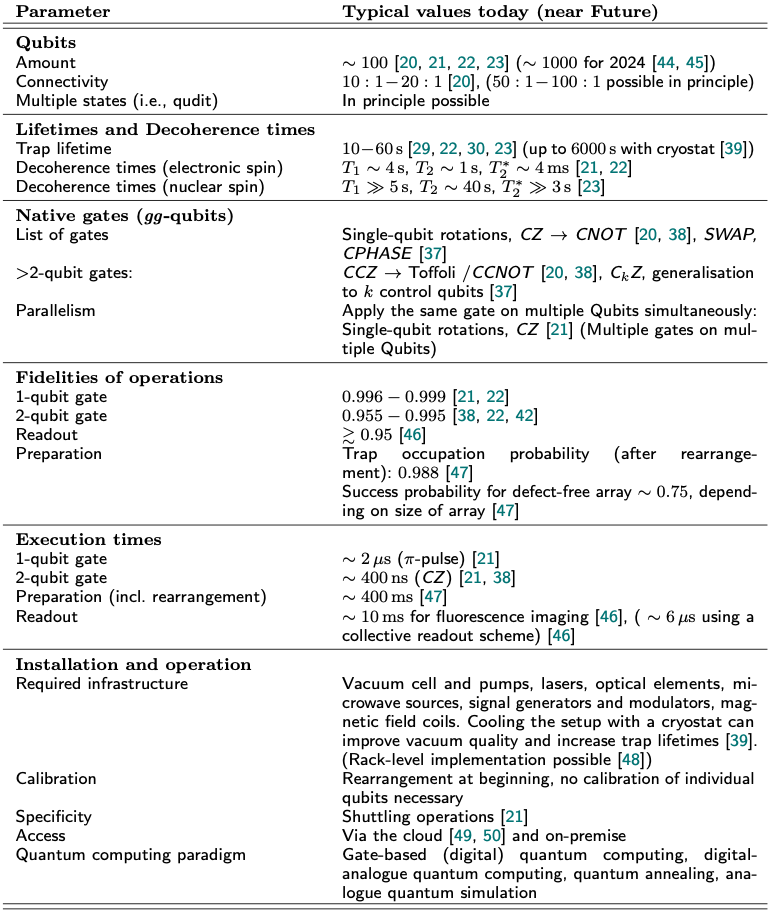
\includegraphics[scale=0.5]{figure1.png}
\end{figure}
\clearpage
\leftline{\large \bfseries 問題}\\
・様々なベンチマークが考案されているが、どの方式のハードウェアを使うかによってvalidityが変化してしまうRef\cite{1}。\\
・中性原子をトラップできる確率は50〜60\%しかないRef\cite{1}\\
・中性原子の並べ替えはやっぱり時間がかかる。\\
・中性原子の並び替えは、動かすqubitの数と動かす距離を最適化しないといけないRef\cite{1}\\
・中性原子方式は測定で原子の状態を捨ててしまうため、もう一度同じ状態を用意するためには最初からやり直さなければならない。\\
\\
\leftline{\large \bfseries 思考}\\
・中性原子の冷却にかかる時間は?\\
・中性原子量子コンピューターではgate操作を同時に行うことが重要であるが、ある適用したいアルゴリズムの回路をどのように分割するかは研究の余地がある。\\
\\
{\Large \bfseries REFERENCES}
\begin{thebibliography}{1}
\vspace{-1.5cm}
  \bibitem{1} Karen Wintersperger, Neutral Atom Quantum Computing Hardware: Performance and End-User Perspective, arXiv:2304.14360v3
  \bibitem{2} Ming-Xin Dong, Highly efficient storage of 25-dimensional photonic qudit in a cold-atom-based quantum memory, arXiv:2301.00999v1
\end{thebibliography}
\vspace{50pt}
\leftline{\bfseries  要調査}
・超伝導やシリコンスピンで取り除かなければならない異質とは何か\\
・中性原子のparasitic chargeとは\\
・中性原子の配列をグラフ理論の点に対応させることで問題を解ける\\
・中性原子の量子ビット再配列方法\\
・analog simulationの可能性\\
・nFT state preparation\\
・feedforwardとmid-circuit measurementの違い\\
・Instataneous Quantum Polynomial\\
・braidingでd以上動かすとどうなるのか\\
・easy intializationとdifficult intializationはどっちがいいのか\\
・toric code in magnetic field(ising model)\\
・bacon-shor code\\
・neutral adn traped ion approaches rely on light scattering for entropy removal\\
・中性原子のmeasurement freeなprotocol\\ 
・Sisyphus cooling\\
・cryostats\\
\\
\end{document}
